\documentclass{article}
\usepackage[margin=1in]{geometry}
\usepackage{amsmath,amsthm,amssymb}
\usepackage{bbm,enumerate,mathtools}
\usepackage{tikz,pgfplots}
\usepackage{chessboard}
\usepackage[hidelinks]{hyperref}
\usepackage{multicol} % Problem 35

\newenvironment{question}{\begin{trivlist}\item[\textbf{Question.}]}{\end{trivlist}}
\newenvironment{note}{\begin{trivlist}\item[\textbf{Note.}]}{\end{trivlist}}
\newenvironment{references}{\begin{trivlist}\item[\textbf{References.}]}{\end{trivlist}}
\newenvironment{related}{\begin{trivlist}\item[\textbf{Related.}]\end{trivlist}\begin{enumerate}}{\end{enumerate}}


\begin{document}
  Suppose two players play a game on a triangular board where they attempt to
  specify the position of markers on the board in a unique way before creating a
  contradiction.
  \begin{enumerate}[(1)]
    \item The first player picks a row on the board, and the second player must
      put a number in the corresponding red box. The number describes how many
      (invisible) markers are in that row.
    \item If the second player believes they have described a unique board, she
      can say so. If (a) she can place markers that satisfy the row labels and
      (b) the other player cannot find another valid way to place the markers,
      then the second player wins.
    \item If the first player believes that the second player's choice creates a
      contradiction, she says so, and the second player has a chance to describe
      a valid board. If the second player can do so, he loses, otherwise he
      wins.
    \item If neither (2) nor (3) occur, then the players reverse roles, and the
    next turn begins from step (1).
  \end{enumerate}
  \begin{figure}[ht!]
    \centering
    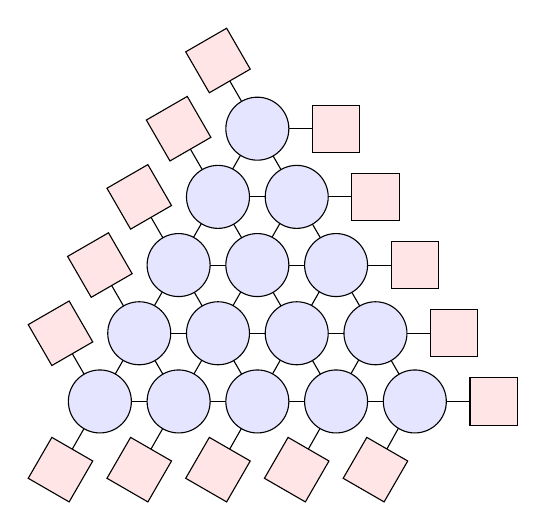
\begin{tikzpicture}
      \def\r{0.3}

      \foreach \x/\y in {1/4, 2/3, 3/2, 4/1, 5/0} {
        \draw (0.5 * \y, {\y * sqrt(3)/2})--(\x + 0.5 * \y, {\y * sqrt(3)/2});
        \draw[fill=red!10]
          (\x - \r + 0.5 * \y, {\y * sqrt(3)/2 - \r}) rectangle
          (\x + \r + 0.5 * \y, {\y * sqrt(3)/2 + \r});
      }

      \foreach \x/\y in {0/-1, 1/-1, 2/-1, 3/-1, 4/-1} {
        % \draw[<-] (0.75 + \x + 0.5 * \y, {\y * sqrt(3)/2})--(1.1 + \x + 0.5 * \y, {\y * sqrt(3)/2});
        \draw (0.5 * \x + 2, {3.5-\x* sqrt(3)/2})--(\x + 0.5 * \y, {\y * sqrt(3)/2});
        \draw[fill=red!10, rotate around={60:({\x + 0.5 * \y}, {\y * sqrt(3)/2})}]
          (\x - \r + 0.5 * \y, {\y * sqrt(3)/2 - \r}) rectangle
          (\x + \r + 0.5 * \y, {\y * sqrt(3)/2 + \r});
      }

      \foreach \x/\y in {-1/1, -1/2, -1/3, -1/4, -1/5} {
        \draw (\y - 1, 0)--(\x + 0.5 * \y, {\y * sqrt(3)/2});
        \draw[fill=red!10, rotate around={-60:({\x + 0.5 * \y}, {\y * sqrt(3)/2})}]
          (\x - \r + 0.5 * \y, {\y * sqrt(3)/2 - \r}) rectangle
          (\x + \r + 0.5 * \y, {\y * sqrt(3)/2 + \r});
      }
      \foreach \x/\y in {
        0/0, 0/1, 0/2, 0/3, 0/4,
        1/0, 1/1, 1/2, 1/3,
        2/0, 2/1, 2/2,
        3/0, 3/1,
        4/0} {
        \draw[fill=blue!10] (\x + 0.5 * \y, {\y * sqrt(3)/2}) circle (0.4cm);
      }
    \end{tikzpicture}
    \caption{
      Examples of all known classes of polygonal chains of length $4$.
    }
  \end{figure}
  \begin{question}
    Which player has a winning strategy?
  \end{question}

  \begin{related}
    \item Does perfect play result in a tie?
    \item How many turns are required under perfect play
      where the winner attempts to win in as few turns as possible, and the
      loser attempts to lose in as many turns as possible?
    \item What if multiple markers can be placed in each row?
    \item How does this generalize to other geometries?
    \item The square analog is essentially the same game under action of the
      torus. Is there an action (besides rotation) that behaves similarly?
  \end{related}
  \begin{references}
    \item Problem 49.
  \end{references}
\end{document}
